\documentclass[english,svgnames,notes=hide,14pt]{beamer}
\usepackage{macros-ohp}

\usepackage{graphics}

\def\presentationtitle{\textcolor{white}{Redescending M-estimators for Robust Regression:\\ A Comparative Analysis based on efficiency factor} }

\title{\large\presentationtitle}
\author{Atiq Ur Rehman\\
		\small Supervised by Insha Ullah and Dost Muhammad\\
		\small 
	}

%Please make sure the tex is compiled twice to have all the images displayed correctly.

%Fill the date or leave it blank to not display it
\date{}


\begin{document}
\thispagestyle{empty}
%\begin{frame}[plain] %put [plain] at the end to get rid of the page number on this page
\begin{frame}
  \titlepage
\end{frame}




\begin{frame}
\frametitle{Contents}
\begin{itemize}
\item Introduction
\item Efficiency factor.
\item Simulation results
\item Summary
\item Q \& A session
\end{itemize}
\end{frame}


\begin{frame}
	\frametitle{Introduction}
	\begin{itemize}
		\item The Ordinary Least Square (OLS) estimation method is used to estimate the regression coefficients.
		\item OLS is sensitive to outliers or to the violation of certain model assumptions. For example, the normality of the residuals.
		\item  Outliers, data points lies far from the majority, could influence the distribution of residuals. Consequently, on the statistical inference procedures involved.
	\end{itemize}
\end{frame}

\begin{frame}{A bit more about the consequences}
\begin{itemize}
    	\item The regression coefficients could be biased and inefficient.
    	\item An insignification regression coefficient could turn to significant because of the presence of outliers in the data. 
    	\item A positive relationship could turn to negative and vice verse.
\end{itemize}
\end{frame}

\begin{frame}{Robust methods}

\begin{itemize}
    \item Robust estimation methods have been proposed: R-estimator, LMS, LTS, S-estimator, M-estimation and others. 
    \item I will be focusing on M-estimation. 
\end{itemize}
\end{frame}

\begin{frame}{OLS Method.}
\textcolor{blue}{Regression model:} 
$$
Y_i = X^{t}_i \beta + \epsilon_{i}.
$$
\textcolor{blue}{Usual OLS estimator:}   
$$
\min_{\beta}\frac{1}{2} \sum_{i = 1}^{n} \epsilon_i^2=\min_{\beta}\frac{1}{2} \sum_{i = 1}^{n} \left(Y_i-X^{t}_i \beta\right)^2
$$
Note that $\rho(\epsilon_{i})=\epsilon_i^2$.
\end{frame}

\begin{frame}{M-estimation.}
The idea is to minimize some other function rather than the squared loss function. For example, Huber chose to minimize
$$
  \rho(\epsilon_{i}) &= \begin{cases} 
      \frac{1}{2} \epsilon^{2}_{i} & |\epsilon_{i}| \leq c \\
      c|\epsilon_{i}| - \frac{1}{2} c^2 & |\epsilon_{i}| > c
   \end{cases},
$$
$$
\psi(\epsilon_{i}) &= \begin{cases} 
\epsilon_{i} & |\epsilon_{i}| \leq c \\
      c~\text{sign}(\epsilon_{i}) & |\epsilon_{i}| > c 
   \end{cases},
$$
where $\psi(.)= \rho^{\prime}(.)$.
% \begin{equation*}
% \rho(\epsilon_{i}/\sigma) = \rho([y_{i} - x^{t}_{i}\beta]/\sigma),
% \end{equation*}
% where $\sigma$ is the scale parameter. To get $\hat{\beta}$, we minimize the above equation w.r.t $\beta$, that is,
% \begin{equation*}
% \hat{\beta} \implies \sum_{i=1}^{n}  (x_{i} \psi(y_{i} - x^{t}_{i}\beta)/\sigma)  = 0, \quad \quad \psi(.)= \rho^{\prime}(.).
% \end{equation*}
\end{frame}

\begin{frame}{Huber $\psi$ and weight functions}
It gives less weight to the outlying observations and thus outliers have less effect on the estimator. 
\begin{figure}
\begin{center}$
\begin{array}{ll}
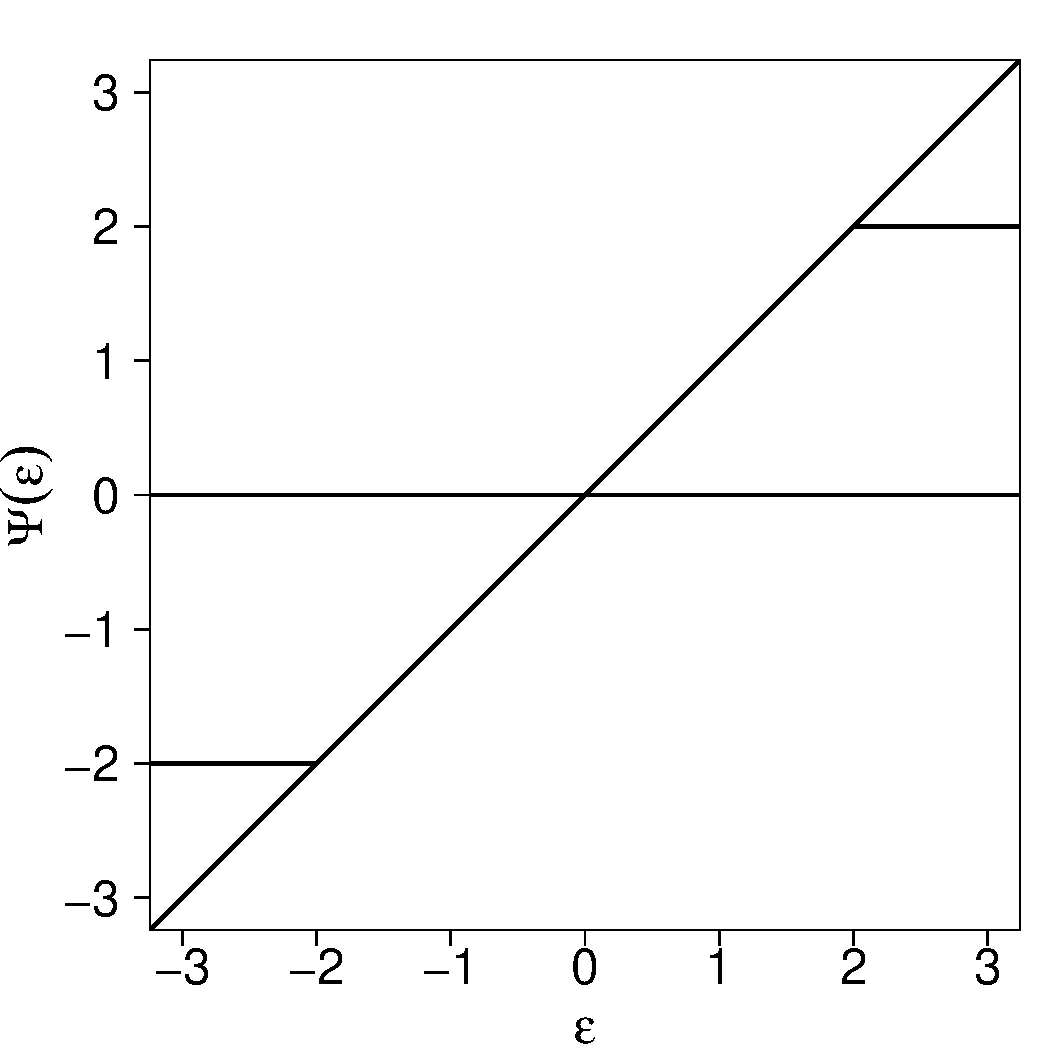
\includegraphics[scale=0.22]{imgs/Hpsi.pdf}
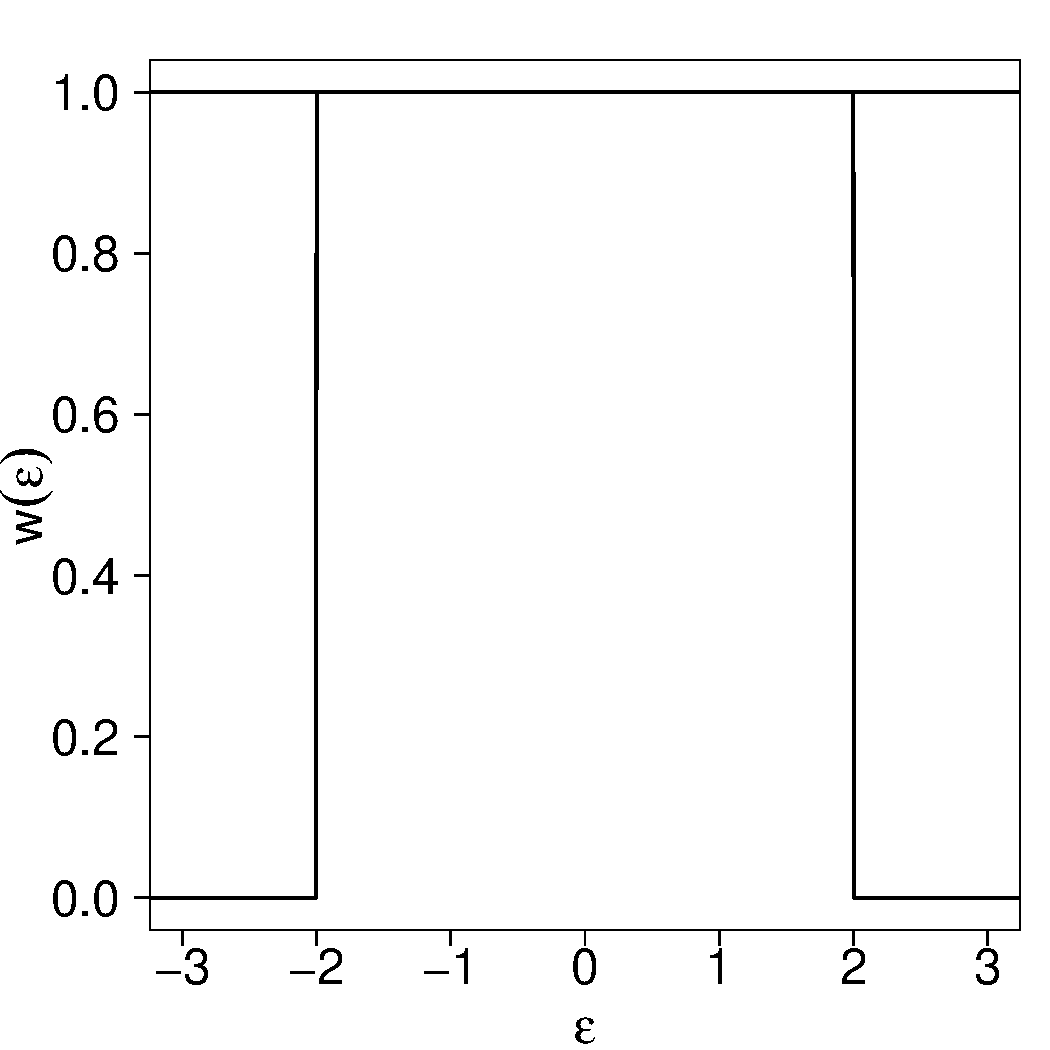
\includegraphics[scale=0.22]{imgs/Hwt.pdf}
\end{array}$
\end{center}
\end{figure}
\end{frame}

\begin{frame}{Redescending M-estimation}
\begin{itemize}
    \item Redescending m-estimator further reduce the influence of the outliers. 
    \item The derivative of $\rho(.)$ = $\psi(.)$ is redescending, that is, $\lim_{\epsilon_{i} \to \infty}  \psi(\epsilon_{i})  = 0$.
    \item rather than $\lim_{\epsilon_{i} \to \infty} \psi(\epsilon_{i})  = \infty$ as in the case of OLS.
    \item $\lim_{\epsilon_{i} \to \infty} \psi(\epsilon_{i})  = c$ as in the case of Huber's proposal.
\end{itemize}
\end{frame}

% Tukey's plots
\begin{frame}{Tukey's dispersion function}
\begin{equation*}
  \rho(\epsilon_{i}) =
   \begin{cases} 
      \frac{c^2}{6} \{1 - [1 - (\frac{\epsilon_{i}}{c})^2 ]^3 \}  & |\epsilon_{i}| \leq c \\
      \frac{c^2}{6} & |\epsilon_{i}| > c
   \end{cases},
\end{equation*}
and
\begin{equation*}
    \psi(\epsilon_{i})&= \begin{cases} 
      \epsilon_{i} [1 - (\frac{\epsilon_{i}}{c})^2 ]^2  & |\epsilon_{i}| \leq c \\
      0 & |\epsilon_{i}| > c
   \end{cases},
\end{equation*}

\end{frame}

\begin{frame}{Tukey's $\psi$ and weight functions}
\begin{figure}
\begin{center}$
\begin{array}{ll}
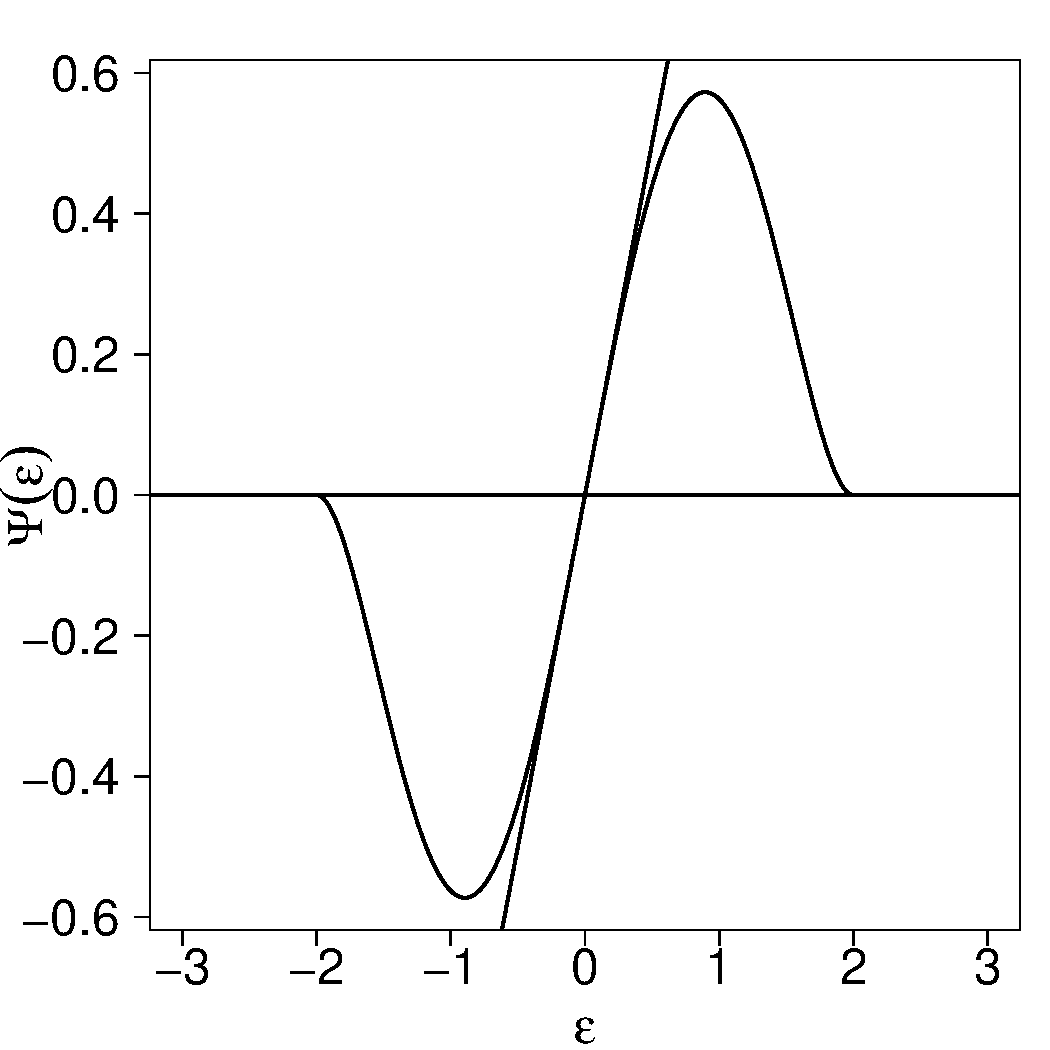
\includegraphics[scale=0.32]{imgs/Tpsi.pdf}
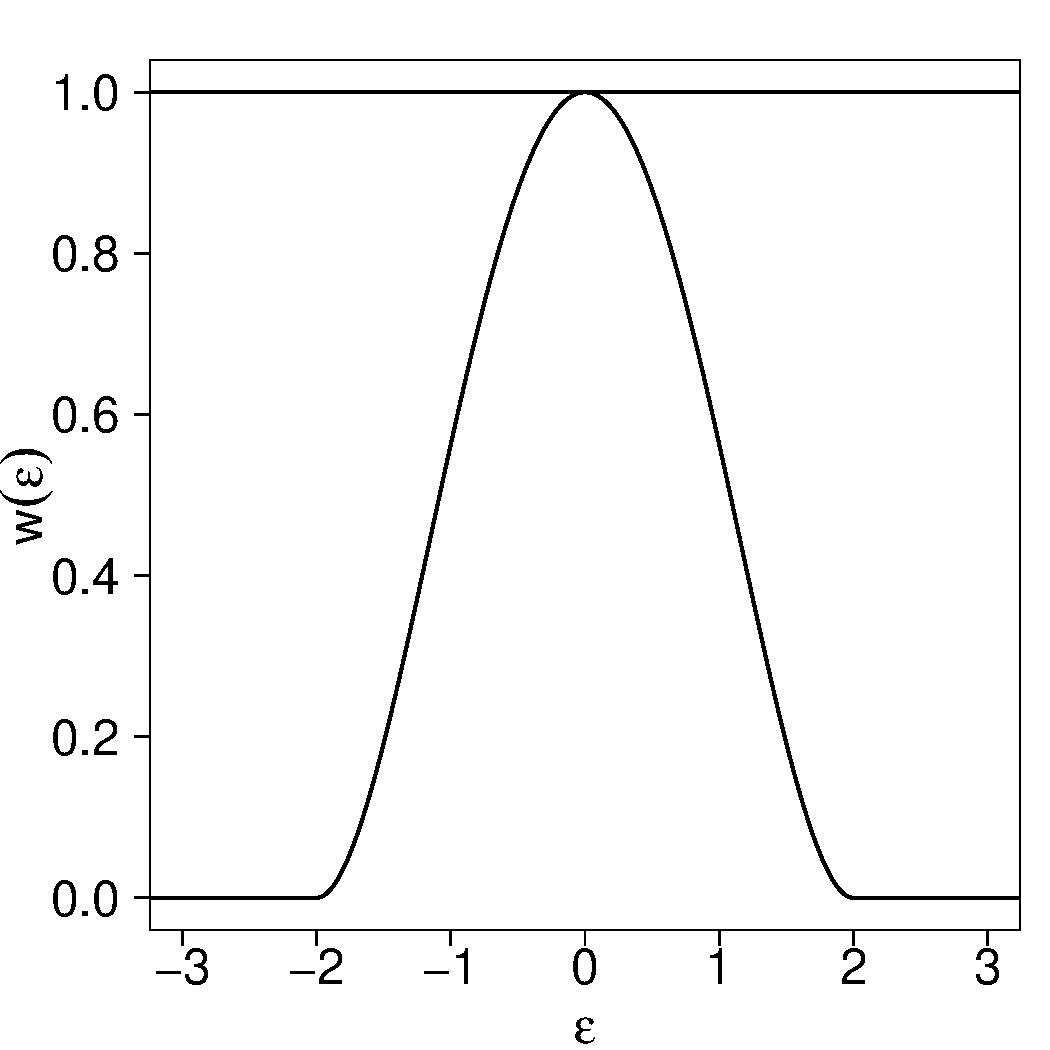
\includegraphics[scale=0.32]{imgs/Twt.pdf}
\end{array}$
\end{center}
\end{figure}
\end{frame}

% Andrew's plots
\begin{frame}{Andrew's dispersion function}
$$
    \rho(\epsilon_{i}) =
   \begin{cases} 
      - c * \cos(\frac{\epsilon_{i}}{c})  & |\epsilon_{i}| \leq c\pi \\
      0 & |\epsilon_{i}| > c\pi
   \end{cases},
$$
and
$$
  \psi(\epsilon_{i})&= \begin{cases} 
      \sin(\frac{\epsilon_{i}}{c})  & |\epsilon_{i}| \leq c\pi \\
      0 & |\epsilon_{i}| > c\pi,
   \end{cases}
$$
\end{frame}
 
\begin{frame}{Andrew's $\psi$ and weight functions}
\begin{figure}
\begin{center}$
\begin{array}{ll}
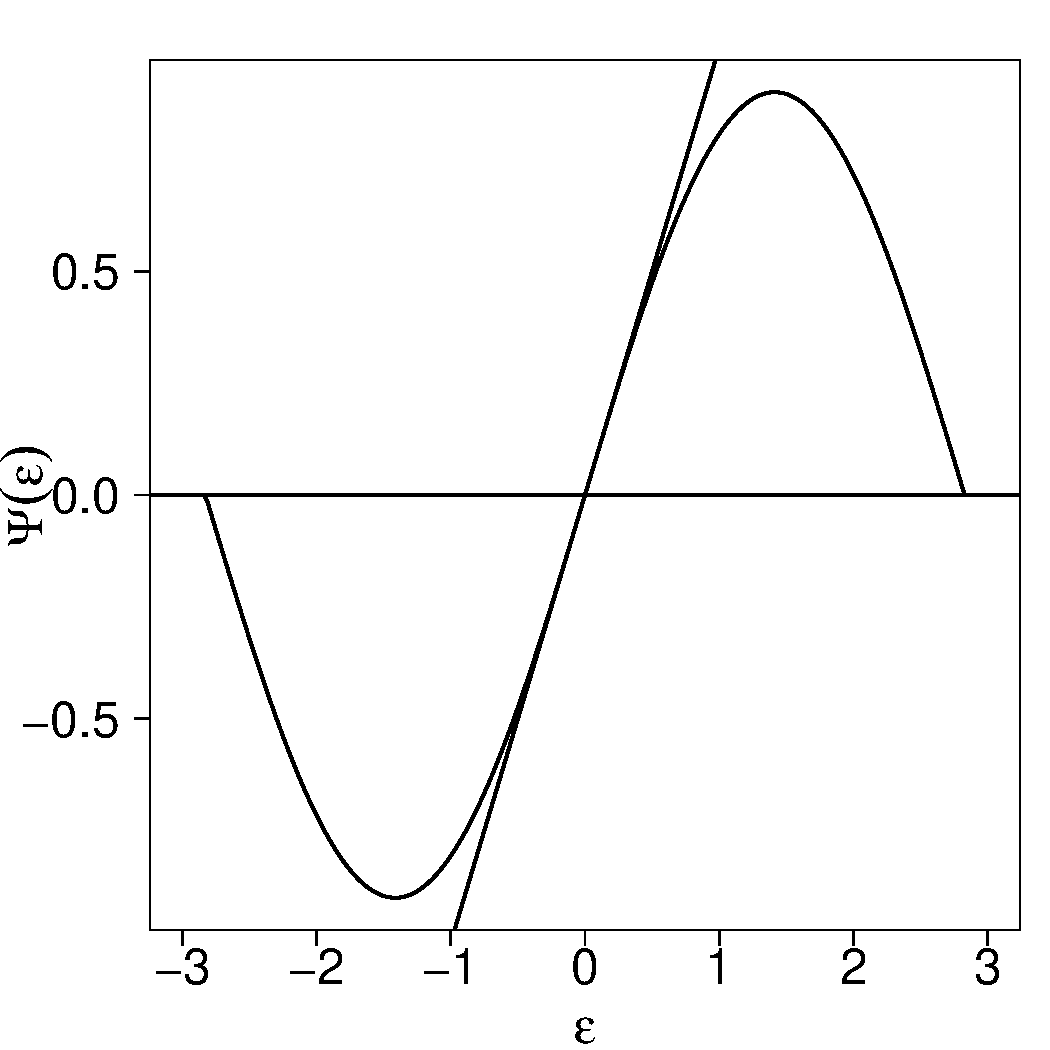
\includegraphics[scale=0.32]{imgs/Apsi.pdf}
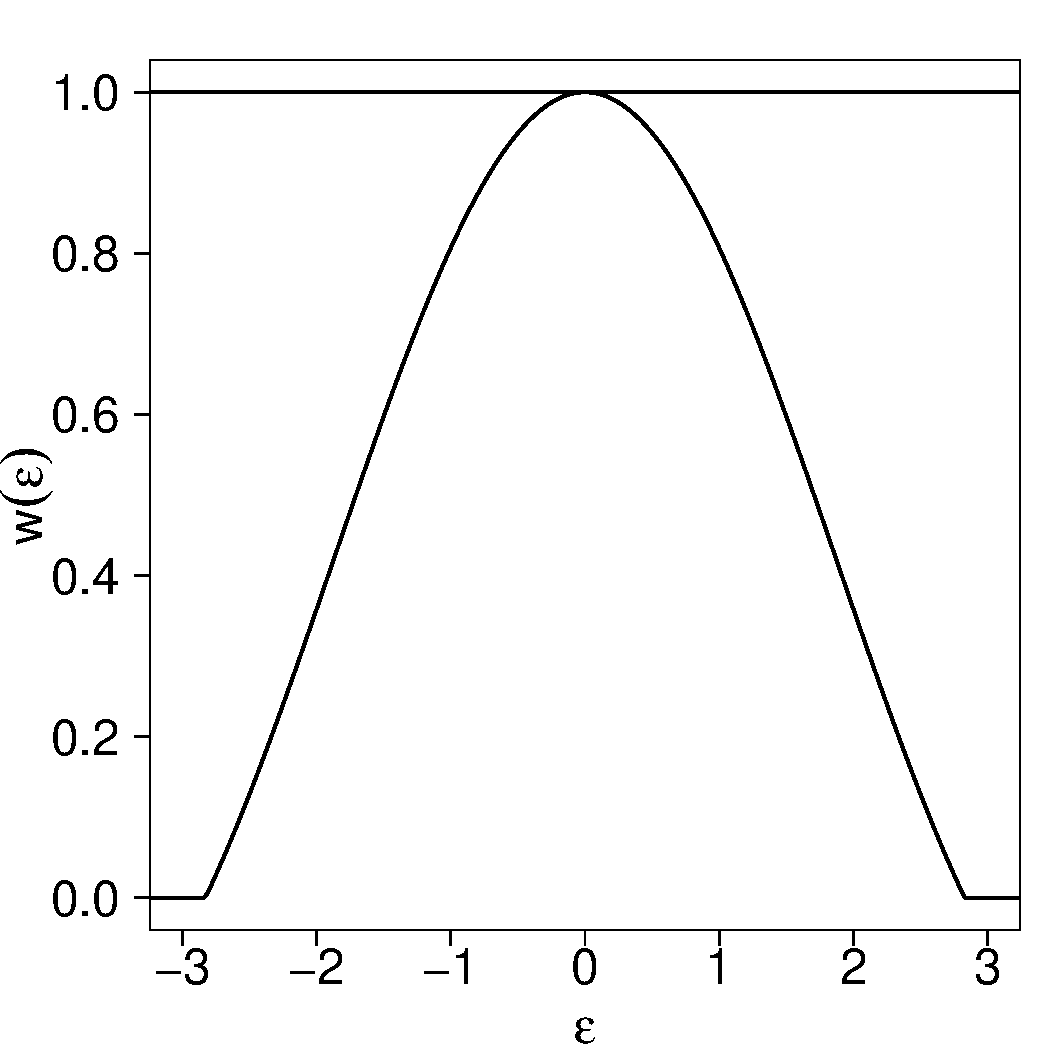
\includegraphics[scale=0.32]{imgs/Awt.pdf}
\end{array}$
\end{center}
\end{figure}
\end{frame}


\begin{frame}{Redescending M-estimator}
\fontsize{14pt}{7.2}\selectfont For example, Andrew's Redescending M-estimator (\textcolor{blue}{Andrew et al. (1972)}), Tukey Redescending M-estimator (\textcolor{blue}{Beaten and Tukey (1974)}), Qadir Redescending M-estimator (\textcolor{blue}{Qadir (1996)}), Modified form of Tukey's biweight function (\textcolor{blue}{Ali and Qadir (2005)}), Insha's redescending M-estimator (\textcolor{blue}{Ullah, Qadir and Ali (2006)}), Alamgir Redescending M-estimator (\textcolor{blue}{Alamgir et al. (2013)}).
\begin{itemize}
    \item The most recent one is \textcolor{blue}{Jiang et al (2018)}. Robust Estimation Using Modified Huber's Functions With New Tails. Technometrics.
\end{itemize} 
\end{frame}

%%%%%%%%%%%%% Huber plots

\begin{frame}{Tuning Constant $c$}
\begin{itemize}
\item All of the M-estimators mentioned above (except OLS) depend on a tuning constant $c > 0$.
\item the value of $c$ need to be chosen without sacrificing efficiency.
\item Default choice in rlm function of R is 1.345 for Huber's M-estimator and 4.685 for Tukey's bisquare.
\item The default choices are not always the best.
\end{itemize}
\end{frame}

\begin{frame}{Data driven approaches}
\begin{itemize}
    \item In the era of Big data one may need to run a model multiple times---each time with a different dataset---it is difficult to choose the best value of $c$ manually 
    \item Automated methods to choose the value of $c$ are required.
    \textcolor{blue}{Wang et al. (2007)} has made tuning constant data-dependent for the Huber's M-estimator.
\end{itemize}
\end{frame}

\begin{frame}{Asymptotic Results.}
$$
 Let \quad \phi_{n}(\theta) = \frac{1}{n S_{n}} \sum_{i=1}^{n} \psi (\frac{Y_{i} - X^{T}_{i}\theta}{S_{n}}) X_{i}
$$
 By Taylor's expansion
\begin{align*}
      \phi_{n}(\hat{\beta}_{n}) =& \phi_{n}(\beta_{0}) + \phi^{\prime}_{n}(\beta_{0})(\hat{\beta}_{n}- \beta_{0}) + \frac{1}{2}(\hat{\beta}_{n}- \beta_{0})^{T} \phi^{\prime \prime}_{n}(\beta_{n}^{\prime})\\  & (\hat{\beta}_{n}- \beta_{0}),
\end{align*}
where $\phi^{\prime}(.)$ and $\phi^{\prime \prime} (.)$ are the first-order and second-order derivatives $\phi(.)$.
\end{frame}

\begin{frame}{}
 As we have $\phi_{n}(\hat{\beta}_{n}) = 0$ and after some algebraic manipulation
\begin{align*}
    \frac{S_{n}}{\sqrt{n} } \sum_{i=1}^{n} \psi (\frac{Y_{i} - X^T_{i}\beta_0}{S_{n}}) X_{i} = & \sqrt{n}(\beta^{\prime}_{n} - \beta_{0}) \frac{1}{ n} \sum_{i=1}^{n}\\ & \psi^{\prime} (\frac{Y_{i} - X^T_\beta_0}{S_{n}}) X^{T}_{i} X_{i} + o_{p}(1)
\end{align*}
\end{frame}

\begin{frame}{}

Since $S_{n} \to \sigma$ as $n \to \infty$, thus

\[
\sqrt{n}(\hat{\beta} - \beta) \sim \mathcal{N} \Big(0, \tau^{-1} \sigma^{2} [E(X^{T}X)]^{-1} \Big)\,,
    \]
where $\tau^{-1} = \frac{[E\psi^{\prime}(\epsilon_{i}/\sigma)]^2}{E \psi^{2}(\epsilon_{i}/\sigma)}=\frac{b^2}{\sigma_\psi^2}$.
The estimate of $b$ can be obtained by
$$b = Pr(|\epsilon_{i}| \leq c)$$ and
$$
\sigma^{2}_{\psi} = \int_{-c}^{c} \psi^{2}(\epsilon_{i}) f(\epsilon_{i}) + c^{2} (1-b)
$$
\end{frame}

\begin{frame}{}
$\hat{\tau}(c)$ for Huber
$$
\hat{\tau}(c) = \frac{[\sum_{i=1}^{n} I(|\hat{\epsilon}_{i}| \leq c)]^2}{n \sum_{i=1}^{n} [I(|\epsilon_{i}| \leq c) \psi^{2} (\hat{\epsilon}_{i}) + c^2 I(|\hat{\epsilon}_{i}| > c)]},
$$
$\hat{\tau}(c)$ for Tukey's
$$
\hat{\tau}(c) = \frac{[\sum_{i=1}^{n} I(|\hat{\epsilon}_{i}| \leq c) \psi^{\prime}(\epsilon_{i})]^2}{n \sum_{i=1}^{n} [I(|\epsilon_{i}| \leq c) \psi^{2} (\hat{\epsilon}_{i})]},
$$
$\hat{\tau}(c)$ for Andrew
$$
\hat{\tau}(c) = \frac{[\sum_{i=1}^{n} I(|\hat{\epsilon}_{i}| \leq c) \psi^{\prime}(\epsilon_{i})]^2}{n \sum_{i=1}^{n} [I(|\epsilon_{i}| \leq c) \psi^{2} (\hat{\epsilon}_{i})]},
$$
\end{frame}


\begin{frame}{$\hat{\tau}$ of Huber for normal and non-normal residuals.}

\begin{figure}
\begin{center}$
\begin{array}{ll}
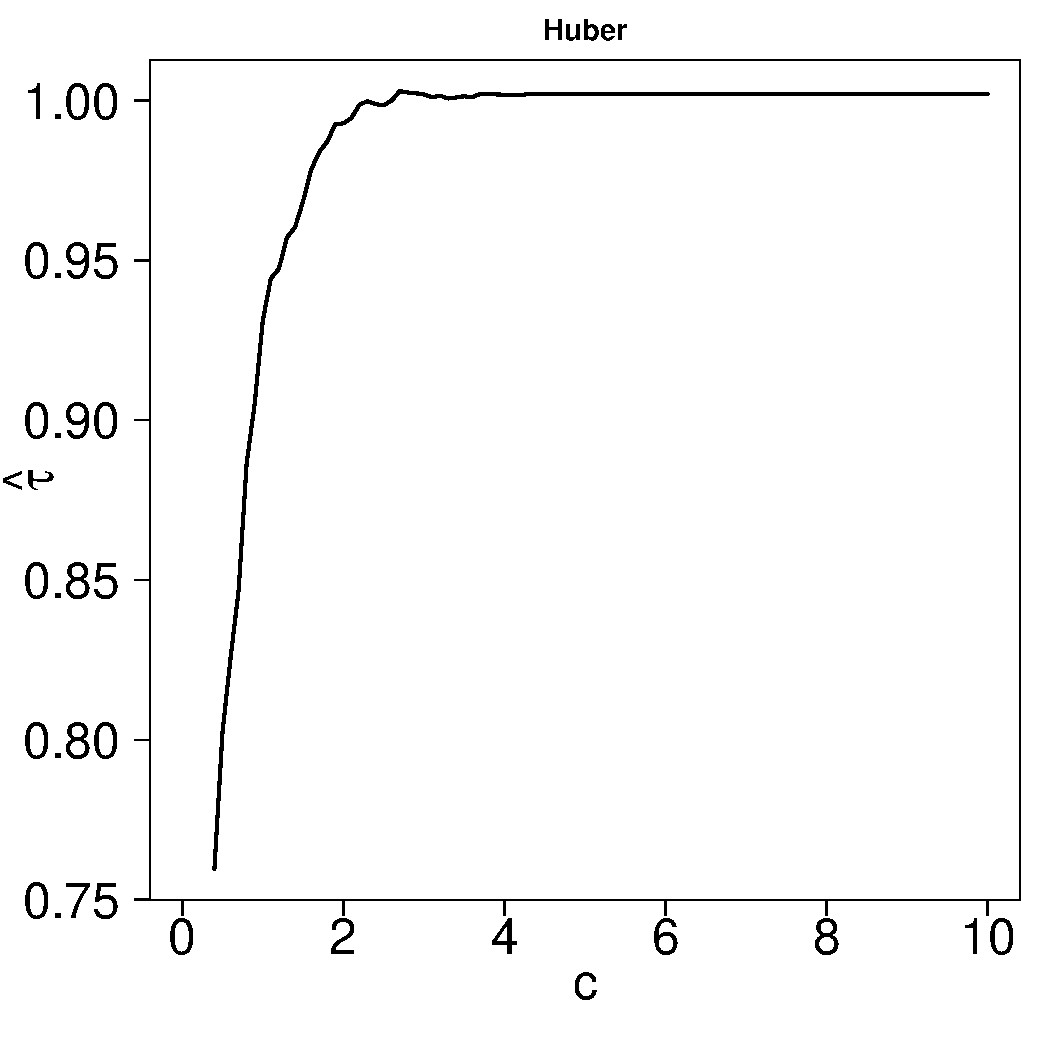
\includegraphics[scale=0.33]{imgs/nTauH.pdf}
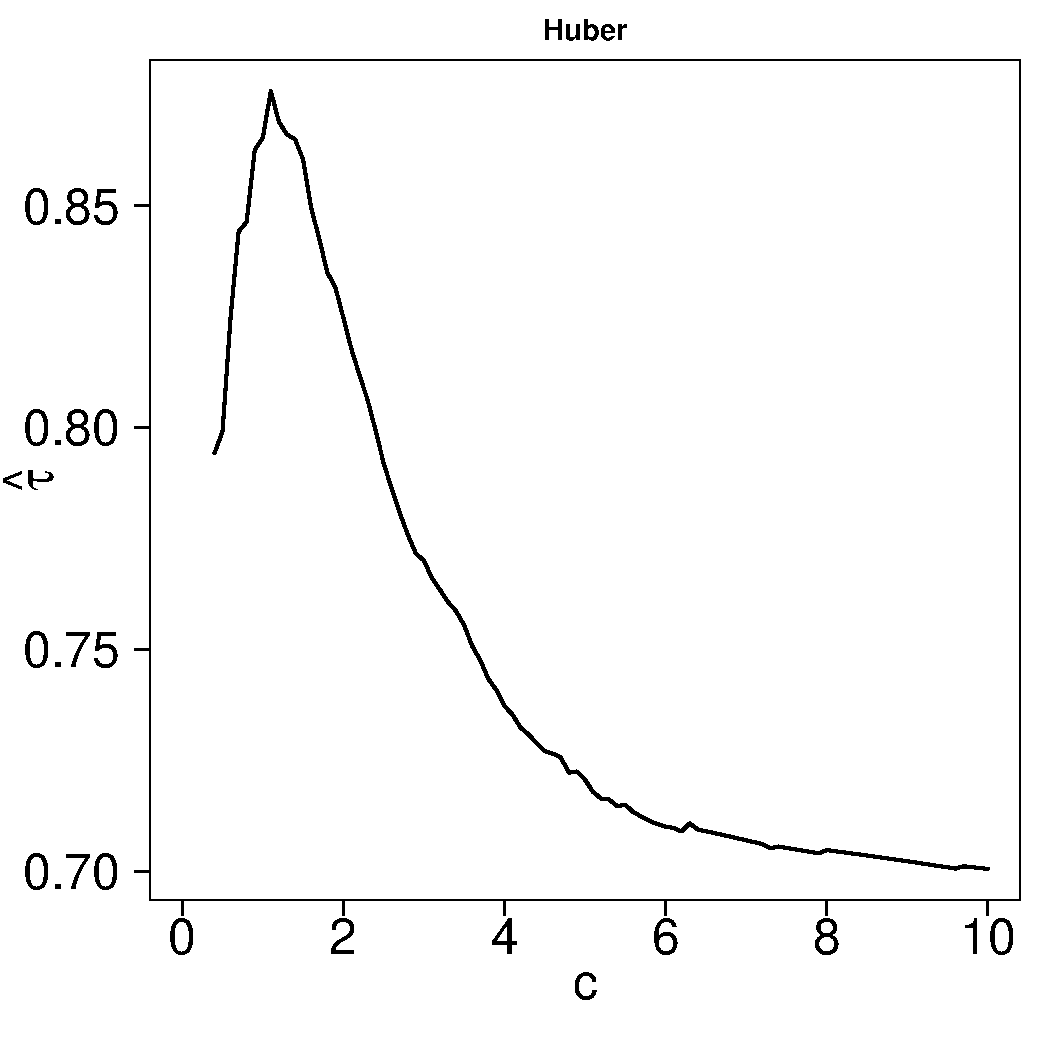
\includegraphics[scale=0.33]{imgs/TauH.pdf}
\end{array}$
\end{center}
\end{figure}
\end{frame}

\begin{frame}{$\hat{\tau}$ of Tukey for normal and non-normal residuals.}

\begin{figure}
\begin{center}$
\begin{array}{ll}
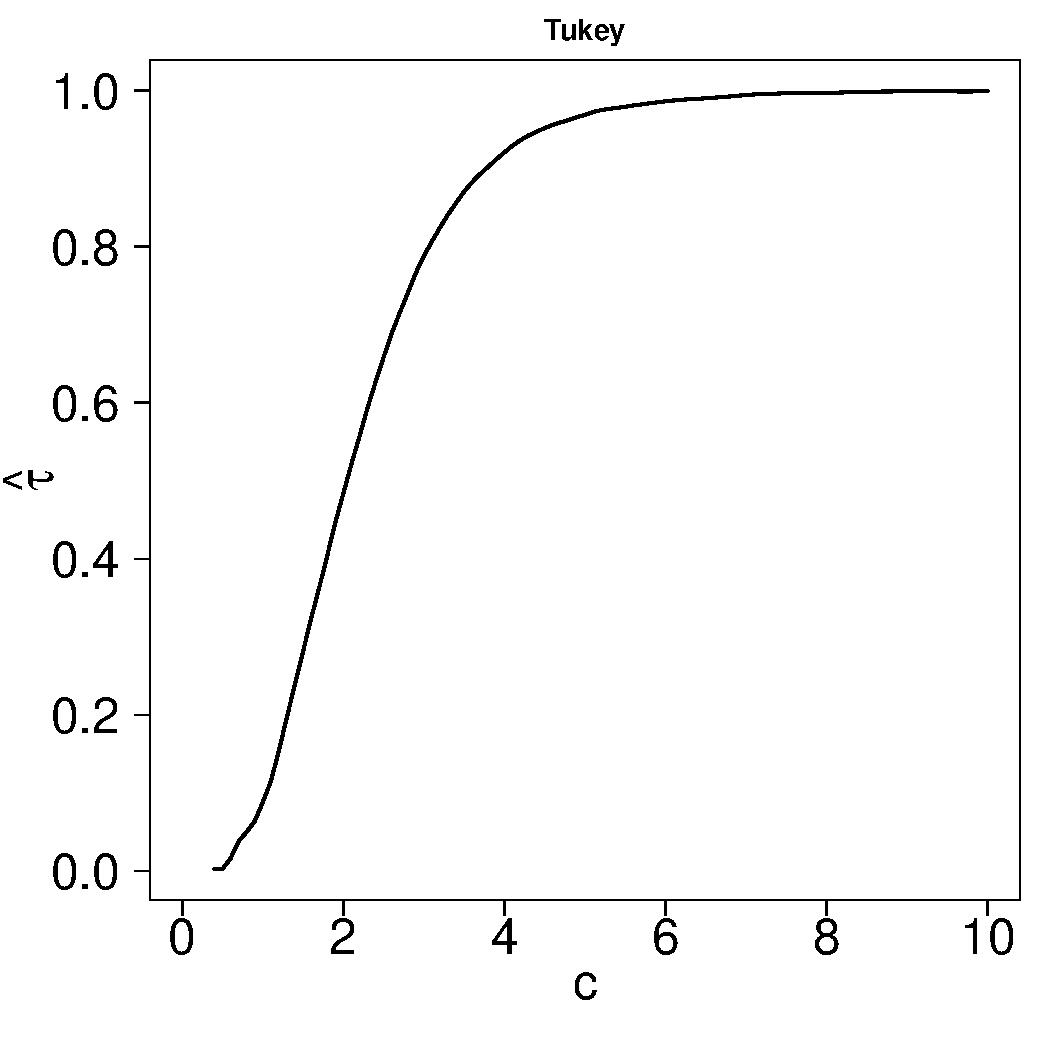
\includegraphics[scale=0.33]{imgs/nTauT1.pdf}
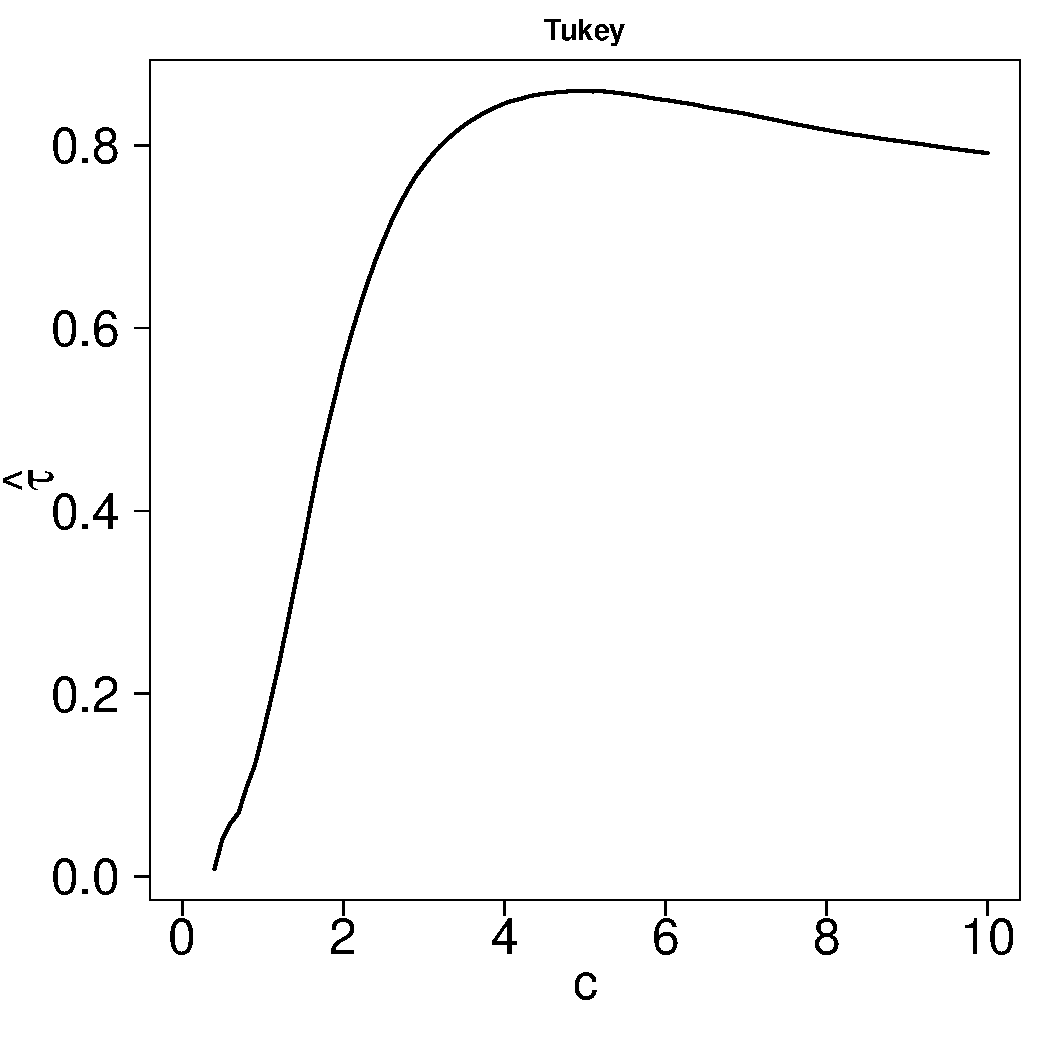
\includegraphics[scale=0.33]{imgs/TauT1.pdf}
\end{array}$
\end{center}
\end{figure}
\end{frame}

\begin{frame}{$\hat{\tau}$ of Andrew for normal and non-normal residuals.}

\begin{figure}
\begin{center}$
\begin{array}{ll}
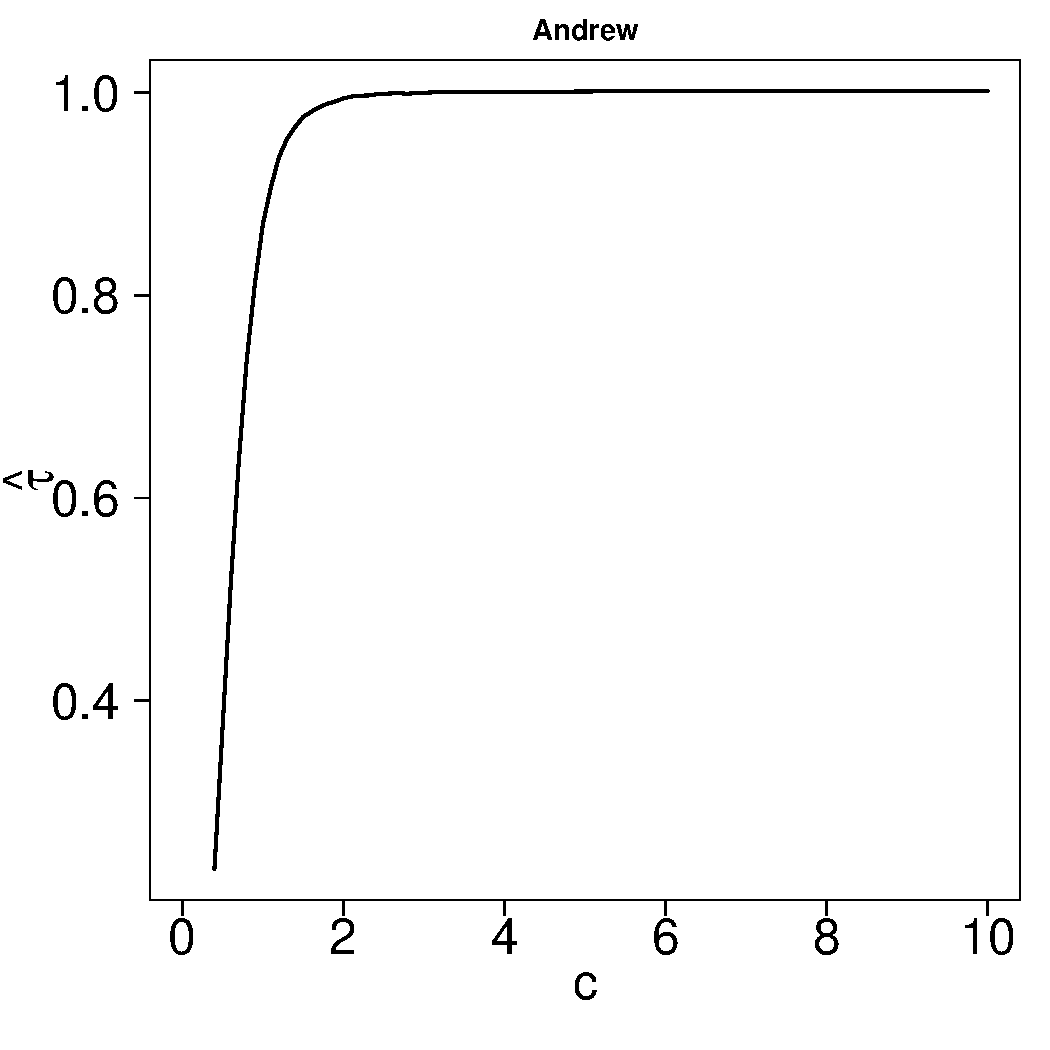
\includegraphics[scale=0.33]{imgs/nTauA.pdf}
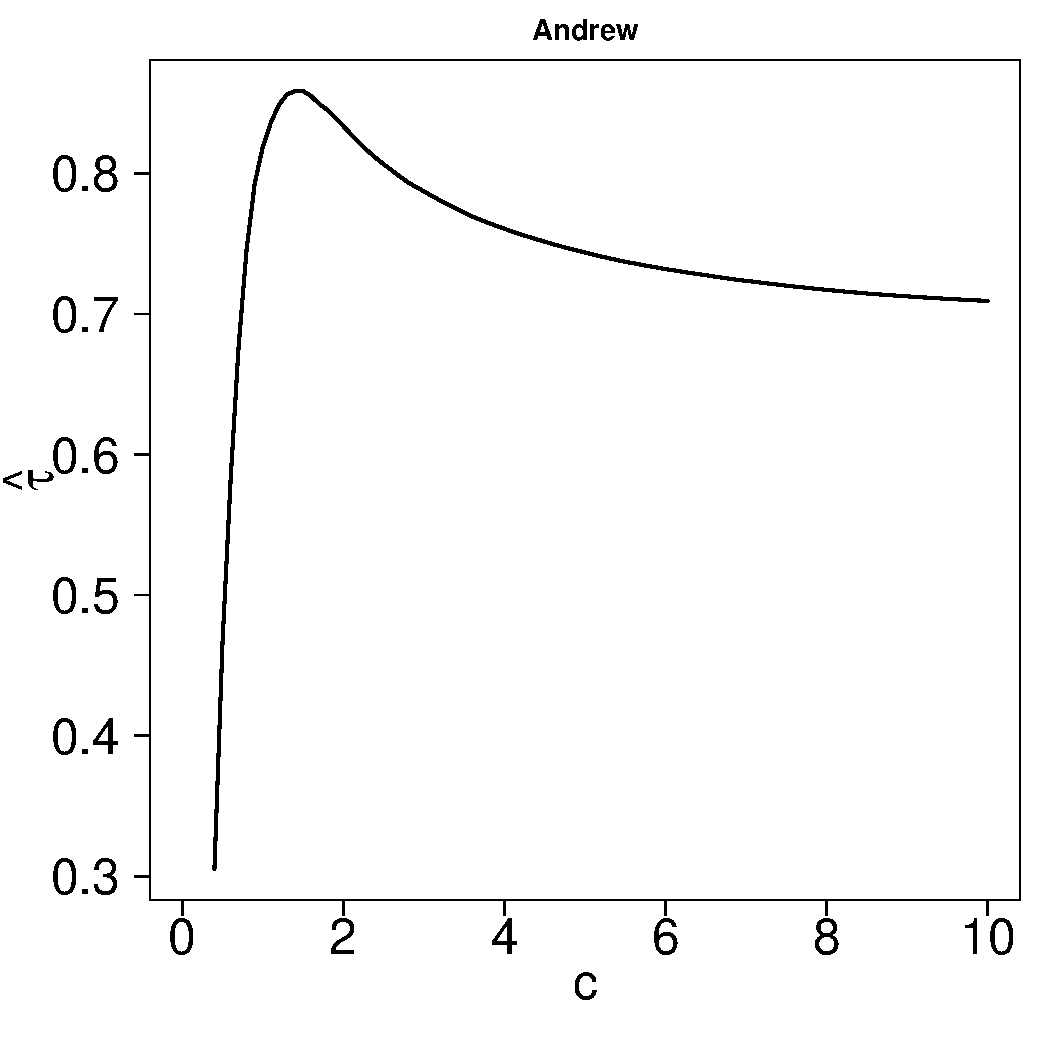
\includegraphics[scale=0.33]{imgs/TauA.pdf}
\end{array}$
\end{center}
\end{figure}
\end{frame}

\begin{frame}{Comparison based on $\hat{\tau}$}
\begin{figure}
\begin{center}
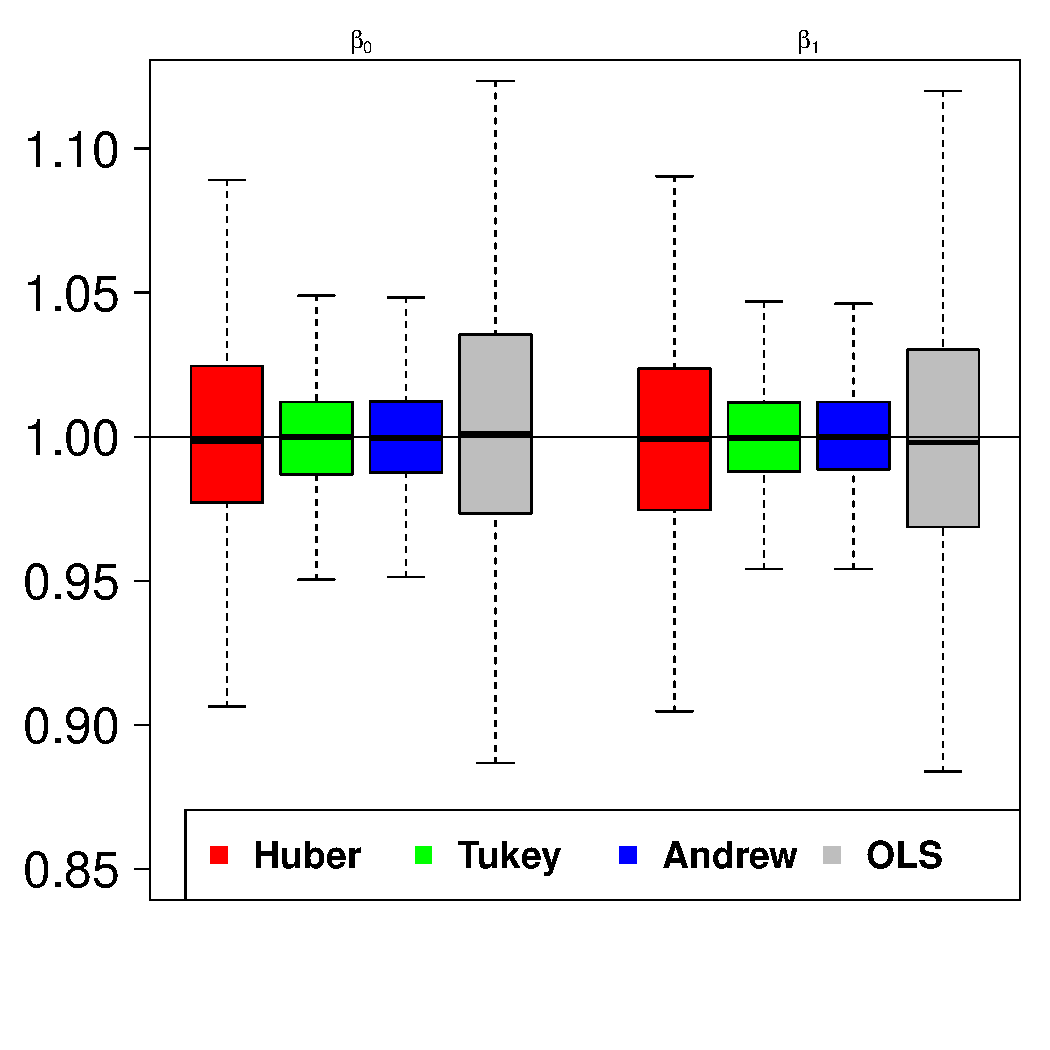
\includegraphics[scale=0.38]{imgs/box.pdf}
\end{center}
\end{figure}
\end{frame}

\begin{frame}{Summary}
\begin{itemize}
    \item Many redescending M-estimator have been proposed.
    \item These estimators depends on the value of c, which is chosen manually. Still no guarantee of efficiency. 
    \item We have used efficiency factor to choose the value of $c$ for redescending M-estimators. 
    \item This efficiency factor helps to choose the best out of many available redescending M-estimators.  
\end{itemize}

    
\end{frame}

\end{document}






%%% Local Variables: 
%%% mode: latex
%%% TeX-PDF-mode: t 
%%% TeX-master: t
%%% End: 